\documentclass[12pt,onehalfspacing]{report}
\usepackage[utf8]{inputenc}
\usepackage{graphicx}
\setcounter{secnumdepth}{0}
\setlength{\parskip}{0pt}

\begin{document}

% Página de título
\thispagestyle{empty}
\begin{center}
  {\large \MakeUppercase{\textbf{DESARROLLO DE UN SISTEMA DE LOCALIZACIÓN Y SEGURIDAD INFANTIL PARA PADRES DE FAMILIA}}}

  \vspace{1in}

  por \\
  FELIX ANDRES ASELA GARCIA (460624)\\
  VALENTINA PEÑUELA NAVAS (451607)\\
  MICHAEL HERNANDEZ MORA (463810)

  \vspace{1.5in}

  El documento se ha elaborado siguiendo las pautas y directrices\\ establecidas para la investigación y desarrollo del proyecto.

  \vspace{2in}

  Bucaramanga, Santander\\       % location
  MARZO 2024                  % date of submission goes here
\end{center}

% Índice
\renewcommand{\contentsname}{Tabla de contenido}
\tableofcontents
\clearpage

\section{Introducción}
\vspace{10pt}
La propuesta que se presenta a continuación tiene como objetivo principal desarrollar un sistema de localización y seguridad infantil para los padres, con la finalidad de brindarles la tranquilidad de conocer la ubicación de sus hijos en todo momento durante el trascurso de un trayecto, y recibir notificaciones al llegar al destino final.\\\\Esta propuesta se enfoca en el diseño y desarrollo de un software especializado en la localización en tiempo real de menores. Este sistema permitirá un seguimiento minucioso de los niños durante trayectos en los que no estén acompañados por sus padres, ofreciendo información detallada sobre su ubicación. El propósito principal de este sistema es aumentar la seguridad de los niños y facilitar la comunicación con los padres.\\\\Para el desarrollo de este sistema se debe identificar 
la situación problema y la pregunta de investigación, ya que estos dos elementos son la base para la construcción del sistema planteado. Una correcta estructuración de la pregunta de investigación nos da a conocer con exactitud el problema que se quiere abordar y, por ende, poder resolverlo.
También se debe definir tanto el objetivo general como los objetivos específicos para el desarrollo del proyecto. Es fundamental destacar que es necesario mencionar las actividades que se deben realizar para cumplir de manera efectiva con cada uno de estos objetivos.\\\\Al mismo tiempo se dan a conocer los antecedentes, donde se presenta el resultado de una búsqueda realizada para identificar y conocer proyectos que ya hayan abordado el mismo contexto del problema que hemos planteado. Finalmente, se expone la justificación del proyecto, que responde a preguntas fundamentales como: ¿Por qué se lleva a cabo? ¿Cuál es el propósito de este proyecto?\\\\

\section{Situación problema}
La seguridad de los menores siempre ha sido una preocupación en nuestra sociedad. Los padres a menudo experimentan miedo al enviar a sus hijos a diversos lugares sin su supervisión directa, como en rutas escolares, al utilizar servicios de transporte como InDrive, cuando son llevados por conocidos, o cuando los niños utilizan el transporte público, todos estos momentos generan una gran inquietud, ya que los padres desean asegurarse de que sus hijos lleguen sanos y salvos a su destino, sin embargo, supervisar el trayecto de los niños resulta difícil, dado que su conocimiento de las calles y rutas es limitado en comparación con el de los adultos.\\\\En cuanto a las rutas escolares, aunque proporcionan cierto nivel de tranquilidad a los padres al ser un transporte designado para llevar a varios niños, no se puede garantizar la seguridad absoluta del niño. Esto se debe a que pueden surgir problemas en la ruta debido a factores externos, lo que implica que siempre exista cierto grado de intranquilidad en cuanto a la protección del menor.\\\\Igualmente, esta situación se repite con otros tipos de transporte, como cuando se envía al niño en el vehículo de otra persona, incluso si es alguien conocido, en estos casos, nunca se puede asegurar completamente que el niño llegará de manera segura a su destino, ya que existen riesgos de imprevistos en la carretera que pueden surgir, de los cuales los padres podrían no estar informados, y el niño debido a su limitado conocimiento sobre la ciudad, no podría comunicar.\\\\La situación se vuelve aún más compleja cuando se trata de transporte público, ya que a veces es la única alternativa disponible para los menores. En estos casos, hay muchos más riesgos, como que el menor se baje en el lugar equivocado o que alguna persona desconocida interfiera y lo dirija hacia otro lugar con intenciones maliciosas.\\\\Considerando la preocupación previamente mencionada por la seguridad de los niños en diferentes medios de transporte, surge la necesidad de reforzar la supervisión de los menores para garantizar su bienestar durante los trayectos. Por lo tanto, la solución tecnológica propuesta busca ofrecer un sistema que permita a los padres supervisar en tiempo real la ubicación y el estado de sus hijos mientras viajan.\\\\Según la problemática plasmada con anterioridad se aborda la siguiente pregunta de investigación:\\

\begin{center}
¿Cómo pueden los padres de familia mejorar la seguridad de sus hijos durante los viajes en diferentes medios de transporte?
\end{center}

\section{Objetivo general}
Desarrollar una aplicación móvil centrada en la seguridad infantil, con el propósito de proporcionar a los padres una herramienta efectiva para monitorizar la ubicación en tiempo real de sus hijos y facilitar la comunicación directa a través de mensajes, contribuyendo así a la promoción de un entorno más seguro y tranquilo para el desarrollo de los niños.

\subsection{Objetivos específicos}
\begin{enumerate}
    \item Identificar los requerimientos funcionales y no funcionales esenciales para el desarrollo de la aplicación, mediante la aplicación de técnicas de especificación como historias de usuario y diagramas de casos de uso. Este proceso seguirá las mejores prácticas de diseño de software, asegurando una comprensión completa de las necesidades y expectativas del usuario.
    \item Diseñar los componentes de la aplicación, abarcando el modelo de base de datos, la arquitectura y la interfaz de usuario. Este diseño se llevará a cabo a través de la elaboración detallada de diagramas de clases y casos de uso, guiados por criterios de calidad en ingeniería del software, con el objetivo de garantizar un desarrollo eficiente y escalable.
    \item Implementar la aplicación propuesta, siguiendo rigurosas buenas prácticas de desarrollo de software y despliegue de aplicaciones. Se prestará especial atención a la documentación de la aplicación y a la incorporación de criterios de seguridad para garantizar la integridad y confidencialidad de los datos de la organización y de los usuarios.
    \item Establecer un mecanismo efectivo de notificación y alerta dentro de la aplicación, permitiendo a los padres recibir información inmediata sobre eventos relevantes, como la entrada o salida de zonas predefinidas por ellos, asegurando así una mayor tranquilidad y respuesta inmediata en situaciones críticas.
\end{enumerate}

\section{Antecedentes}
Los sistemas de localización han experimentado un crecimiento exponencial en la última década, con una amplia gama de aplicaciones en diversos sectores \cite{survey_localization}. En el ámbito de la seguridad infantil, la localización en tiempo real se ha convertido en una herramienta fundamental para proteger a los más pequeños, a lo largo del tiempo han existido herramientas que han direccionado su enfoque en este campo \cite{indoor_localization}.\\\\
Herramientas como “Life360”, una plataforma de localización familiar con más de 30 millones de usuarios en 200 países destaca por su interfaz intuitiva, funciones robustas como seguimiento en tiempo real, historial de ubicaciones, alertas de seguridad y geocercas, y planes gratuitos y premium que se ajustan a diversas necesidades. Su éxito se debe a su facilidad de uso para todas las edades, funciones que van más allá de la simple localización, opciones para diferentes presupuestos y una estrategia de marketing eficaz que genera confianza en la marca \cite{life360}, Google Family Link, una aplicación de gestión parental integrada al ecosistema de Google, que facilita la supervisión de los hijos para las familias que ya usan sus productos. Ofrece funciones como localización en tiempo real, control de aplicaciones y tiempo de pantalla, y configuración de permisos, permitiendo a los padres establecer límites de uso, aprobar o bloquear aplicaciones y juegos, y controlar el tiempo frente a la pantalla. Su éxito se debe a la integración con Google, su enfoque en la seguridad y el control parental, su gratuidad y su preinstalación en dispositivos Android, lo que la hace accesible y fácil de usar para todas las familias \cite{google_family_link} y FamilyTime se destaca como una solución integral de seguridad infantil, ofreciendo no solo localización en tiempo real, sino también funciones avanzadas de control parental como filtro de contenido web, control de aplicaciones y tiempo de pantalla, y monitoreo de redes sociales. Además, la aplicación proporciona informes detallados sobre la actividad de los niños en línea, permitiendo a los padres estar al tanto de lo que hacen sus hijos en internet. Su éxito se basa en estas funciones que van más allá de las opciones básicas, en sus informes detallados de actividad y en su enfoque en la seguridad y el control parental, convirtiéndola en una opción atractiva para padres que buscan proteger a sus hijos en línea \cite{familytime}.\\\\
Diversas aplicaciones se han adentrado en el área de la seguridad y localización infantil, el éxito de estas aplicaciones depende de varios factores como las funcionalidades, una amplia gama de funciones útiles, la usabilidad, una interfaz intuitiva para padres e hijos, los costos, planes accesibles, la seguridad, protección robusta de datos y el marketing, una estrategia eficaz para generar confianza, mientras que el fracaso puede ocurrir por la falta de funcionalidades, funciones básicas o poco atractivas, dificultad de uso, interfaz compleja, costo elevados, planes inaccesibles, problemas de seguridad, vulnerabilidades en la plataforma y marketing deficiente, estrategias ineficaces para conectar con el público objetivo \cite{child_safety}.\\\\
Las aplicaciones de localización para la seguridad infantil son herramientas valiosas que pueden ayudar a los padres a proteger a sus hijos. Sin embargo, no son una solución mágica y deben usarse con responsabilidad. También es importante recordar que las aplicaciones de localización no son un sustituto de la supervisión parental directa.\\\\
Hay que tener en cuenta que los niños por su vulnerabilidad física y mental son un grupo especialmente susceptible a la inseguridad. Esta problemática se presenta en diversos contextos uno de estos es el transporte. El camino a la escuela puede ser un escenario de acoso por parte de otros niños o incluso adultos. Un estudio de la UNESCO reveló que 1 de cada 3 estudiantes en el mundo ha sido víctima de acoso escolar \cite{unesco_bullying}, los niños pueden perderse con mayor facilidad en el transporte público, sobre todo cuando no están en compañía de un adulto, por estas razones la seguridad de los niños en el transporte es un problema complejo que requiere un enfoque multisectorial. los gobiernos, las empresas de transporte, las escuelas y las familias deben trabajar juntos para crear un entorno de transporte seguro para todos los niños, las herramientas antes mencionadas y MaxiDrive buscan brindar su aporte a la mejora de esta problemática.


\section{Justificación}
Los padres hoy en día se pueden ver limitados debido a diversas circunstancias de actos tales como llevar a sus hijos a la escuela o a diferentes puntos de la ciudad, teniendo en cuenta además la peligrosidad de enviar a un menor solo en el transporte público o distintos tipos de movilidad.\\\\
Los padres entonces se ven obligados a contratar servicios de transporte que aseguren la movilidad de los infantes, como única alternativa a esta problemática, sin embargo, tiene factores de riesgo y es que, una vez despedidos los niños y en el transporte, los padres no tienen manera de hacer un seguimiento a sus hijos.\\\\ 
El software aquí propuesto tiene como objetivo dar solución a este problema esencialmente brindando a los padres de familia una manera de recibir información referente a la localización de su hijo, haciendo un seguimiento obteniendo la ubicación GPS en tiempo real o recibiendo notificaciones en su dispositivo cuando por el niño llega inicia su trayecto y cuando lo finaliza.\\\\
La implementación de esta aplicación no solo sirve como un método para los padres de estar más al pendiente de la situación de sus hijos cuando estos no están a su alcance sino también ayuda a respaldar el trabajo de los transportistas, al establecer un cierto nivel de vigilancia por parte de los padres.

\section{Marco referencial}
Para investigar los recursos necesitados para la creación del proyecto, se realizó una investigación bibliográfica sobre los instrumentos necesarios para la elaboración del sistema de localización. La base del análisis en general se basó en la situación problema la cual ya fue descrita. Las herramientas y técnicas para utilizar son: Flutter para desarrollar la interfaz de usuario móvil, permitiendo crear aplicaciones multiplataforma con interfaces atractivas y fluidas. Flask y Echo serán utilizados en la creación de APIs para facilitar la comunicación entre la aplicación móvil y el servidor, garantizando un entorno de desarrollo robusto y escalable. ASP.NET Core será utilizado como alternativa para la creación de APIs según las necesidades específicas del proyecto, mientras que MySQL y PostgreSQL se encargarán del almacenamiento de datos relacionados con la localización y seguridad infantil. Herramientas como Jenkins automatizarán tareas de integración y despliegue continuos, Ubuntu será el sistema operativo base para los servidores, Docker asegurará entornos de desarrollo y despliegue consistentes, GitHub gestionará el control de versiones y colaboración, y Azure facilitará el despliegue y gestión de la aplicación en la nube.

\section{Marco conceptual}
A continuación, se presentan fragmentos del significado de las herramientas mencionadas anteriormente, cubriendo áreas como Bases de Datos, desarrollo de software e ingeniería de software.\\\\
\textbf{Aplicaciones móviles}\\
Para dar inicio al marco conceptual sería prudente iniciar con la base en al que se desarrolla el proyecto, las aplicaciones móviles. \\\\Una aplicación móvil es una aplicación de software desarrollada específicamente para su uso en pequeños dispositivos informáticos inalámbricos, como teléfonos inteligentes y tabletas, en lugar de computadoras de escritorio o portátiles.\\\\Las aplicaciones móviles a veces se clasifican según si están basadas en la web o son aplicaciones nativas, que se crean específicamente para una plataforma determinada. Tambien existe una tercera categoría, las aplicaciones híbridas, que combina elementos de aplicaciones nativas y web.\\\\En la era digital actual, las aplicaciones móviles son una parte esencial de la vida diaria de la mayoría de las personas. Desde las redes sociales y el entretenimiento hasta la productividad y los negocios, las aplicaciones móviles juegan un papel vital en la forma en que interactuamos con la tecnología. 
Las aplicaciones móviles están diseñadas para ejecutarse en sistemas operativos móviles específicos, como iOS, Android y Windows Phone. Cuando se descarga e instala una aplicación móvil en un dispositivo, se almacena en la memoria del dispositivo y se inicia con el sistema operativo del dispositivo.\\\\Cuando un usuario abre una aplicación móvil, la aplicación se comunica con el sistema operativo del dispositivo y otros componentes de software integrados para acceder al hardware y los servicios del dispositivo, como la cámara, el GPS y la conexión a Internet. A continuación, la aplicación utiliza esta información para proporcionar sus funciones y servicios específicos al usuario.\\\\
Dicho esto la aplicación desarrollada en este proyecto tiene interacciones con mucha información, información que e almacena en diversas bases de datos.\\\\
\textbf{Bases de datos}\\
Una base de datos es una recopilación organizada de información o datos estructurados, que normalmente se almacena de forma electrónica en un sistema informático. Normalmente, una base de datos está controlada por un sistema de gestión de bases de datos (DBMS). En conjunto, los datos y el DBMS, junto con las aplicaciones asociadas a ellos, reciben el nombre de sistema de bases de datos, abreviado normalmente a simplemente base de datos.
Los datos de los tipos más comunes de bases de datos en funcionamiento actualmente se suelen utilizar como estructuras de filas y columnas en una serie de tablas para aumentar la eficacia del procesamiento y la consulta de datos. Así, se puede acceder, gestionar, modificar, actualizar, controlar y organizar fácilmente los datos. La mayoría de las bases de datos utilizan un lenguaje de consulta estructurada (SQL) para escribir y consultar datos.
Las bases de datos son definitivamente una de las tecnologías más importantes de la actualidad y es que tienen considerables ventajas:

\begin{enumerate}
    \item Evita datos repetidos o duplicados
    \item Aumenta la productividad
    \item Permiten ingresar datos ilimitados
    \item Compartir datos globalmente
    \item Centralizar la información
\end{enumerate}
En el caso de una aplicación como la planteada el manejo de la información es importante en extremo para el manejo de la vigilancia y monitoreo de los padres a los niños relacionando usuarios, almacenando información de los conductores, puesto que cada base de datos tiene diferentes ventajas y características está planteado que se puedan usar distintas bases de datos según las necesidades, por ejemplo, MySQL para los usuarios, mongodb para mensajes o PostgreSQL para manejo de rutas interno. Lo más importante es que sin importar que base de dato se use esta debe estar debidamente configurada para un buen funcionamiento.\\\\
\textbf{Copias de seguridad/back ups}\\
Una vez revisada la importancia de las bases de datos sobra mencionar la importancia de la información que estas contienen y debido a esto esta información deben estar asegurada.\\\\
las copias de seguridad o back ups usualmente se realizan en medios distintos a los originales, esto puede ser tanto en servicios externos de nube como aws o azure que presten este servicio o en servidores físicos locales separados, de esta manera en casos de accidentes de corrupción, perdida o destrucción, la información perdida pueda ser respaldada y recuperada evitando los problemas que conlleva la perdida de información.
Para el caso de un sistema de localización y seguridad infantil como el planteado la seguridad de la información manejada es imprescindible por lo que se debe establecer una estrategia de copia de seguridad robusta y resistente a incidentes que mantenga la integridad de la información.\\\\Queda claro entonces que es esencial una política de copias de seguridad efectiva garantizando la continuidad de la prestación del servicio.\\\\
\textbf{Framework de desarrollo}\\
Un framework es un conjunto de reglas y convenciones que se usan para desarrollar software de manera más eficiente y rápida. Estos marcos de trabajo se emplean para ahorrar tiempo y esfuerzo en el desarrollo de aplicaciones, ya que proporcionan una estructura básica que se puede utilizar como punto de partida. Además, los frameworks también ofrecen soluciones a problemas comunes en el desarrollo de software, lo que significa que los desarrolladores pueden centrarse en las funcionalidades específicas de su aplicación en lugar de perder tiempo resolviendo problemas técnicos. Los frameworks tienen una gran serie de ventajas y funciones como:
\begin{enumerate}
    \item \textbf{\textit{Mejora la eficiencia:}} Estandariza los procesos y las metodologías, lo que permite a los equipos trabajar de manera más eficiente y productiva.
    \item \textbf{\textit{Acelera el tiempo de desarrollo:}} Al tener una estructura clara y establecida, el desarrollo de proyectos se acelera, lo que permite alcanzar los objetivos más rápidamente.
    \item \textbf{\textit{Facilita la colaboración:}} Permite a los equipos trabajar juntos de manera más efectiva, lo que mejora la colaboración y la comunicación.
    \item \textbf{\textit{Mejora la calidad:}} Al tener un marco de trabajo claro y estandarizado, los resultados finales son más coherentes y de mejor calidad.
    \item \textbf{\textit{Aumenta la flexibilidad:}} Permite a los equipos adaptarse a cambios y ajustarse a las necesidades del proyecto de manera más eficiente.
\end{enumerate}



\section{Marco Tecnológico }
Este proyecto de desarrollo de un sistema de localización y seguridad infantil para padres se basa en la integración de diversas tecnologías para lograr su implementación efectiva. Se utilizarán herramientas modernas y versátiles que permitan la creación de una aplicación móvil funcional. A continuación, se describen las tecnologías principales que se emplearán en este sistema:\\\\
\textbf{Flutter}\\
Flutter es un marco de desarrollo de código abierto creado por Google, diseñado para la construcción de aplicaciones móviles multiplataforma de alta calidad. Con Flutter, los desarrolladores pueden crear interfaces de usuario atractivas y fluidas que se ejecutan de manera nativa en dispositivos iOS y Android. Su enfoque en la velocidad de desarrollo y la facilidad de mantenimiento lo convierte en una opción popular para proyectos móviles. En este proyecto específico, Flutter será utilizado como la herramienta principal para desarrollar la interfaz de usuario de una aplicación dedicada a la localización y seguridad infantil.\\\\
\textbf{ASP.NET Core}\\
Para desarrollar las APIs que facilitarán la comunicación entre la aplicación móvil y el servidor, se optará por ASP.NET Core, una plataforma desarrollada por Microsoft. Este marco de trabajo ofrece un entorno sólido y escalable para la creación de APIs utilizando el lenguaje de programación C#. ASP.NET Core provee una solución completa para el desarrollo web, que incluye funcionalidades como enrutamiento, middleware y compatibilidad con servicios web RESTful.\\\\
\textbf{Flask y Echo}\\
Además de ASP.NET Core, se utilizarán Flask y Echo como alternativas para desarrollar APIs, dependiendo de las necesidades particulares del proyecto. Flask es un marco de trabajo liviano y flexible en Python que permite crear APIs de manera rápida y sencilla. Por otro lado, Echo es un marco de trabajo en Go diseñado para construir APIs web altamente eficientes. La elección de cada marco se basa en los requisitos específicos del proyecto y las preferencias del equipo de desarrollo. Cada uno de estos marcos ha sido previamente seleccionado para cumplir con las necesidades del proyecto, ya que ofrecen características avanzadas y un enfoque modular que facilita tanto el desarrollo inicial como el mantenimiento continuo de la aplicación móvil.
Para almacenar datos relacionados con la localización y la seguridad infantil, se emplearán sistemas de gestión de bases de datos relacionales como MySQL y PostgreSQL. Ambos sistemas proporcionan funcionalidades avanzadas que se ajustan a las necesidades del proyecto y garantizan un alto nivel de fiabilidad y escalabilidad.\\\\
\textbf{MySQL}\\
MySQL es una popular base de datos relacional de código abierto ampliamente adoptada en aplicaciones web y móviles. Reconocida por su capacidad para gestionar grandes conjuntos de datos y su rendimiento eficiente, MySQL representa una elección confiable para almacenar información crucial relacionada con la seguridad y ubicación de los niños. Su facilidad de uso y su amplia disponibilidad en el mercado lo convierten en una opción preferida entre los desarrolladores.\\\\
\textbf{PostgreSQL}\\
PostgreSQL es un sistema de gestión de bases de datos relacional de código abierto reconocido por su robustez y capacidad para manejar cargas de trabajo complejas. Ofrece soporte para características avanzadas como transacciones ACID, integridad referencial y replicación, convirtiéndose en una opción óptima para aplicaciones que requieren un alto nivel de fiabilidad y disponibilidad de datos. Su arquitectura flexible y su conjunto completo de herramientas lo posicionan como una solución poderosa para el almacenamiento de datos en el ámbito de la seguridad infantil.\\\\
\textbf{Jenkins}\\
Jenkins es una herramienta de código abierto utilizada para la automatización de la integración y despliegue continuo (CI/CD). Con Jenkins, es factible automatizar diversas tareas como la compilación de código, pruebas unitarias, análisis estático y despliegue de aplicaciones. Su función es crucial en el proceso de desarrollo al facilitar la entrega constante de cambios en el software de manera eficiente y segura.\\\\
\textbf{Ubuntu}\\
Ubuntu, un sistema operativo basado en Linux, ha sido seleccionado como la plataforma para alojar los servidores de la aplicación de seguridad y localización infantil. Conocido por su estabilidad, seguridad y facilidad de uso, Ubuntu es una opción popular para el alojamiento de aplicaciones y servicios web. Su amplio respaldo por parte de la comunidad y las actualizaciones regulares garantizan un entorno confiable y robusto para ejecutar la infraestructura de servidores necesaria para respaldar el funcionamiento de la aplicación. En este proyecto, Ubuntu será el sistema operativo principal elegido para proporcionar un entorno seguro y estable para la implementación y ejecución de la aplicación de seguridad y localización infantil.\\\\
\textbf{Docker y Docker Compose}\\
Docker es una plataforma de código abierto diseñada para la creación, distribución y ejecución de aplicaciones en contenedores. Estos contenedores proporcionan un entorno aislado y liviano, permitiendo que los desarrolladores empaqueten aplicaciones junto con todas sus dependencias y las ejecuten de manera coherente en diferentes entornos. Por otro lado, Docker Compose es una herramienta que simplifica la definición y gestión de aplicaciones que constan de múltiples contenedores. En este proyecto, se emplearán Docker y Docker Compose para establecer un entorno de desarrollo y despliegue uniforme y reproducible.\\\\
\textbf{GitHub}\\
GitHub es una plataforma colaborativa de desarrollo que sirve para alojar y administrar proyectos de software utilizando el sistema de control de versiones Git. A través de GitHub, equipos de desarrollo pueden colaborar de manera eficiente en la creación de software, hacer un seguimiento de los cambios realizados, gestionar problemas y solicitudes de modificación, así como automatizar procesos de integración continua. En este proyecto, GitHub será utilizado como el repositorio central para almacenar el código fuente y manejar el flujo de trabajo de desarrollo.\\\\
\textbf{Azure}\\
Azure es una plataforma de computación en la nube desarrollada por Microsoft, que ofrece una variedad de servicios y herramientas para el desarrollo, despliegue y gestión de aplicaciones en la nube. Entre sus servicios se incluyen alojamiento web, bases de datos, análisis de datos, servicios de inteligencia artificial, entre otros. En este proyecto, se empleará Azure para implementar y administrar la aplicación de localización y seguridad infantil en un entorno de nube seguro y escalable.

\section{Metodología}
El sistema de información se desarrollará utilizando la metodología “Modelado por Prototipos ", pero primero se debe comprender cómo funciona dicho método. El modelo de prototipos se basa en el diseño rápido, el cual está centrado en una imagen de las propiedades del software que serán visibles para el usuario. El prototipo debe construirse rápidamente usando los programas apropiados con un uso mínimo de recursos. Dicho diseño lleva a la creación de un prototipo temprano, o innovación, que es valorado por el usuario final para un feedback; como resultado, se refinan las necesidades del sistema de información que se desarrollará. La interacción tiene lugar cuando el prototipo se acopla para complacer las necesidades del usuario. Gracias a esto, el desarrollador puede comprender lo que se debe hacer y, al mismo tiempo, permite que el cliente vea los resultados rápidamente. [8]
El prototipado es una metodología que implica la creación de versiones preliminares de un producto o sistema con el objetivo de visualizar y probar conceptos antes de la implementación completa. A continuación, se describen los pasos típicos de la metodología de prototipado:
\begin{enumerate}
    \item \textbf{\textit{Recolección y refinamiento de Requisitos:}} Se recopilan y documentan los requisitos del sistema, identificando las funcionalidades clave y las necesidades de los usuarios. Este paso es fundamental para asegurar que el prototipo aborde de manera efectiva los aspectos esenciales del producto o sistema.
    \item \textbf{\textit{Diseño Rápido:}} En esta fase, se crea un diseño preliminar que sirve como base para el desarrollo del prototipo. Se establece la estructura general y la interfaz de usuario, proporcionando una visión inicial del producto.
    \item \textbf{\textit{Construcción del prototipo:}} Aquí, se construye la versión inicial del producto o sistema, centrándose en la implementación de las funcionalidades clave. Este prototipo inicial sirve como una representación tangible de la visión conceptual.
    \item \textbf{\textit{Evaluación del prototipo por el cliente:}} El prototipo se somete a pruebas exhaustivas para identificar posibles problemas y recopilar retroalimentación de los usuarios. Esta fase es crucial para mejorar la funcionalidad y corregir errores antes de avanzar en el desarrollo.
    \item \textbf{\textit{Refinamiento del prototipo:}} Se realizan ajustes y mejoras en el diseño y la funcionalidad del prototipo en función de la retroalimentación recibida. Esta iteración permite perfeccionar la solución y abordar cualquier área de mejora identificada durante las pruebas.
    \item \textbf{\textit{Producto de Ingeniería:}} Se lleva a cabo la creación del producto final basándose en el prototipo perfeccionado. Utilizando el prototipo refinado como guía, se procede con el desarrollo completo del software. Una vez que el producto está completamente desarrollado, se lanza al mercado, y se inicia la vigilancia continua para evaluar su desempeño y aceptación en el mercado.\cite{beneficios_prototipado}
\end{enumerate}
La elección de la metodología de "Modelado por Prototipos" resulta altamente beneficiosa en el desarrollo de software destinado a empresas dedicadas a la recuperación de hierro. Esta metodología facilita una iteración continua del diseño y la funcionalidad, asegurando así que el sistema de información cumpla con los requisitos específicos de los clientes. Al ofrecer el software de manera gratuita a empresas con recursos limitados, la metodología de "Modelado por Prototipos" se convierte en un recurso valioso para agilizar el desarrollo y prevenir posibles problemas de implementación. En resumen, se presenta como una opción muy adecuada para la construcción de aplicaciones de este tipo, garantizando la facilidad de manipulación y mantenimiento a largo plazo del sistema de información, además de satisfacer las necesidades particulares de las empresas recuperadoras de hierro.\\\\
\begin{figure}[h]
  \centering
  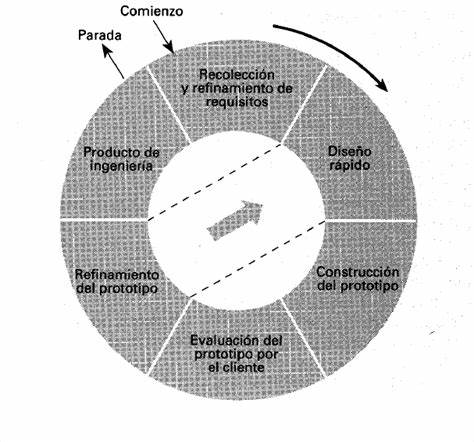
\includegraphics[width=0.5\textwidth]{PrototipadoImg}
  \caption{Metodología Modelado por Prototipos. \cite{modelo_prototipos}}
  \label{fig:prototipado}
\end{figure}\\
Establecidos los conceptos, se sienta una base sólida para la creación de un software destinado a facilitar la gestión de los procesos de recuperación de hierro en las empresas del sector. Los principios y teorías presentados en este marco proporcionan una comprensión profunda de los desafíos y oportunidades que enfrenta esta industria, lo que facilita la identificación precisa de las necesidades específicas que el software debe abordar. Además, la decisión de emplear la metodología de "Modelado por Prototipos" en el desarrollo del software asegura una iteración continua del diseño y la funcionalidad, lo que contribuiría a una mayor adaptabilidad a las necesidades del usuario final.


% Referencias
\bibliographystyle{unsrt}
\bibliography{referencias}

\end{document}
